\section{Direct Serendipity Space}
Serendipity element have the same accuracy of approximation with 
classical tensor product element while use smaller number of degrees of freedom.
However, the classical serendipity space suffer from poor approximation
on quadrilaterals. We define local shape functions directly
on quadrilaterals according to~\cite{directSerendipity}.
$H^1$ and $H(\text{div})$ conforming direct mixed finite elemenent space
are constructed with the direct serendipity function space.

To begin with, we introduce some notations and distance auxilliary functions. 
Let $\mathbb{P}_r(\omega)$ denote the space of polynomials of degree up to $r$
on $\omega \subset \mathbb{R}^d$. The dimension of $\mathbb{P}_r$ can be
calculated as
\begin{equation}\label{eq:dimpolynomial}
		  \text{dim}\mathbb{P}_r(\mathbb{R}^d) = \begin{pmatrix}
r+2 \\
2
		  \end{pmatrix} = \frac{(r+d)!}{r!d!}.
\end{equation}
We define the linear polynomial $\lambda_i(\mathbf{x})$ giving the
distance of $\mathbf{x}\in \mathbb{R}^2$ to edge $e_i$ as
\begin{equation}\label{eq:distancelambda}
		  \lambda_i(\mathbf{x}) = -(\mathbf{x}-\mathbf{x}^*_i)\cdot \pmb{\nu}_i, \quad i = 0,1,2,3,
\end{equation}
where $\mathbf{x}^*_i \in e_i$  is any point on the edge $e_i$. The value of
distance function $\lambda_i$ keeps positive as long as $\pmb{x}$ is in the
interior of the quadrilateral. We define two additional distance functions giving 
the distance of $\mathbf{x} \in \mathbb{R}^2$ to diagonal line $d_{i}$ 
joining $v_i$ with $v_{i+2}$, $i\in{0,1}$.
Let $\mathbf{\nu}_{d,i}$ be the unit normal vector to the diagonal line 
$d_{i}$. The direction of the $\mathbf{\nu}_{d,i}$ is defined by 
counterclockwise rotating of the vector pointing from $v_i$ to $v_{i+2}$.
The resulting diagonal distance function is defined as
\begin{equation}\label{eq:distancelambdad}
		  \lambda_{d,i}(\mathbf{x}) = -(\mathbf{x} - \mathbf{x}^*_{d,i}) \cdot \pmb{\nu}_{d,i}, 
		  \quad i=1,2,
\end{equation}
where $\mathbf{x}^*_{d,i}$ is any point on the diagonal line $d_{i}$. For
simplicity, we use corner $v_i$ in later computation.

Now we present set of nodal basis functions in first and second
order direct serendipity space $\mathcal{DS}_1$ and $\mathcal{DS}_2$
defined by ~\cite{directSerendipity}.

\subsection{Direct Serendipity Space $\mathcal{DS}_2$}
We supplement polynomial space $\mathbb{P}_r(E), r\geq 2$ 
with two linearly independent
functions, $\phi_{s,1}(\mathbf{x})$ and $\phi_{s,2}(\mathbf{x})$. We denote
the supplemental function space as $\mathbb{S}_r^{\mathcal{DS}}(E) = 
\text{span}\{\phi_{s,1},\phi_{s,2}\}, \quad r\geq 2$. We present the second order 
direct serendipity
space as
\begin{equation}\label{eq:definitionds2}
		  \mathcal{DS}_2(E) = \mathbb{P}_2(E) \oplus \mathbb{S}_2^{\mathcal{DS}}(E).
\end{equation}
The supplemental functions are defined as
\begin{equation}\label{eq:defsuppfunc}
		  \phi_{s,i}(\mathbf{x}) = \lambda_{i+1}(\mathbf{x}) \lambda_{i+2}(\mathbf{x}) R_{i,i+2}(\mathbf{x}), \quad i\in\{1,2\},
\end{equation}
where $i$ is in the sense of modulo. We use a simple definition for rational
function $R_{i,i+2}$ as
\begin{equation}\label{eq:defR}
		  R_{i,i+2}(\mathbf{x}) = \frac{\lambda_{i}(\mathbf{x}) - \lambda_{i+2}(\mathbf{x})}{\lambda_i(\mathbf{x}) + \lambda_{i+2}(\mathbf{x})},
\end{equation}
which satisfies the conditions as
\begin{equation}\label{eq:Rproperty}
		  R_{i,i+2}|_{e_i} = -1, \quad R_{i,i+2}|_{e_{i+2}} = 1.
\end{equation}
We continue to define
\begin{equation}\label{eq:def}
		  R_i(\mathbf{x}) = \frac{1}{2} \Big(1 - (-1)^{\floor*{i/2}} R_{i, i+2}(\mathbf{x})\Big) 
		  = \frac{\lambda_{i+2}(\mathbf{x})}{\lambda_i(\mathbf{x}) + \lambda_{i+2}(\mathbf{x})},
\end{equation}
where $i$ is understood $\Mod{2}$. Here, $R_i|_{e_i} = 1$, and
$R_i|_{e_{i+2}} = 0$ by definition. In Figure~\ref{fig:R0}, we
draw $R_0$ on a general quadrilateral, which evaluates $1$ 
on the edge $e_0$, and evaluates $0$ on the opposite edge $e_2$.
\begin{figure}[ht]
\centering\small
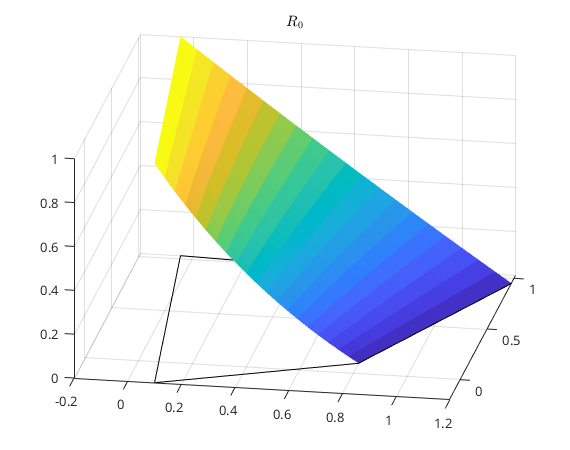
\includegraphics[width=5.5cm,height=4cm]{chapters/pics/R0_1.png}
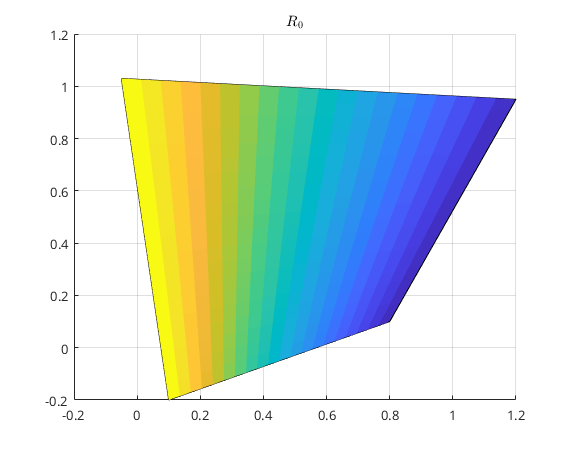
\includegraphics[width=5.5cm,height=4cm]{chapters/pics/R0_2.png}
		  \caption{Rational function $R_0$.}
		  \label{fig:R0}
\end{figure}

The edge nodal basis functions for $\mathcal{DS}_2$ are constructed as
\begin{equation}\label{eq:edgebasisds2}
		  \varphi_{e,i}(\mathbf{x}) = \frac{\lambda_{i+1}(\mathbf{x})\lambda_{i+3}(\mathbf{x})R_i(\mathbf{x})}
		  {\lambda_{i+1}(\mathbf{x}_{e,i})\lambda_{i+3}(\mathbf{x}_{e,i})R_i(\mathbf{x}_{e,i})},
\end{equation}
where $\mathbf{x}_{e,i}$ is the middle point of the edge $e_i$, the $i$ index is
understood in the sense of modulo of $4$. In Figure~\ref{fig:phie0}, we present
$\varphi_{e,0}$ on a general quadrilateral.
\begin{figure}[ht]
\centering\small
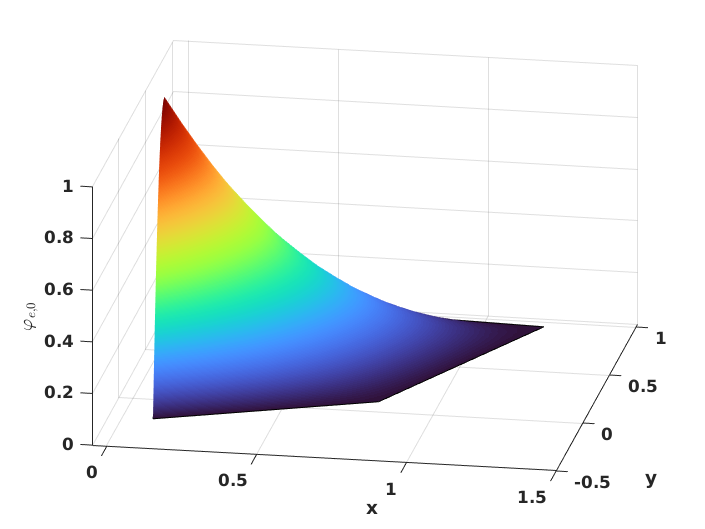
\includegraphics[width=5.5cm,height=4cm]{chapters/pics/phie0_1.png}
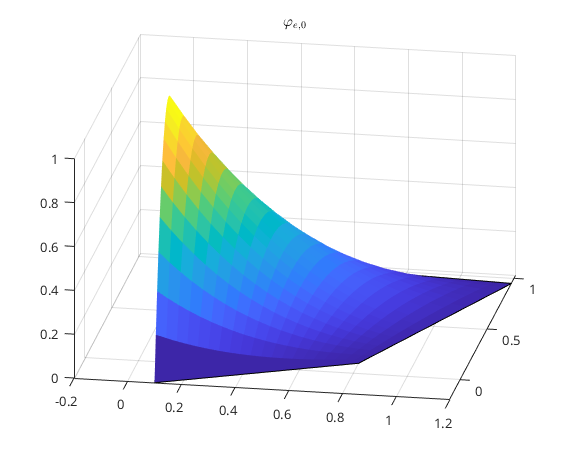
\includegraphics[width=5.5cm,height=4cm]{chapters/pics/phie0_2.png}
		  \caption{Edge nodal basis function $\varphi_{e,0}$ in $\mathcal{DS}_2$.}
		  \label{fig:phie0}
\end{figure}

The vertex nodal basis functions for $\mathcal{DS}_2$ are constructed as
\begin{equation}\label{eq:vertexbasisds2}
		  \varphi_{v,i}(\mathbf{x}) = \frac{\lambda_{i+2}(\mathbf{x}) \lambda_{i+3}(\mathbf{x}) - 
		  \sum_{k=i}^{i+1}\lambda_{i+2}(\mathbf{x}_{e,i})\lambda_{i+3}(\mathbf{x}_{e,i})\varphi_{e,i}(\mathbf{x})}
		  {\lambda_{i+2}(\mathbf{x}_{v,i}) \lambda_{i+3}(\mathbf{x}_{v,i}) - 
		  \sum_{k=i}^{i+1}\lambda_{i+2}(\mathbf{x}_{e,i})\lambda_{i+3}(\mathbf{x}_{e,i})\varphi_{e,i}(\mathbf{x}_{v,i})},
\end{equation}
where $\mathbf{x}_{v,i}$ is the coordinates of the vertex node $v_i$. The $i$ index
is understood in the sence of module of $4$ as well. In Figure~\ref{fig:phiv0}, we 
show $\varphi_{v,0}$ on a general quadrilateral.
\begin{figure}[ht]
\centering\small
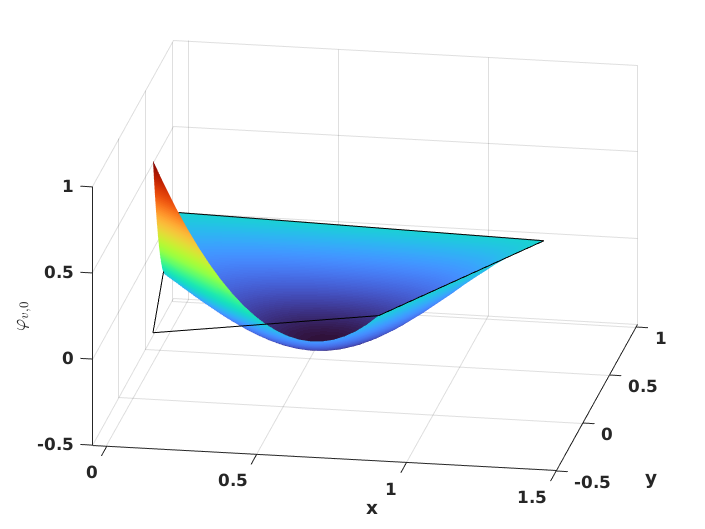
\includegraphics[width=5.5cm,height=4cm]{chapters/pics/phiv0_1.png}
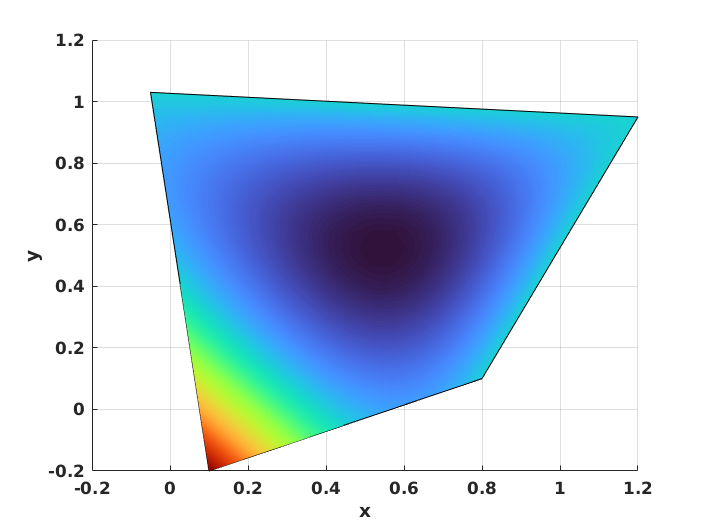
\includegraphics[width=5.5cm,height=4cm]{chapters/pics/phiv0_2.png}
		  \caption{Vertex nodal basis function $\varphi_{v,0}$ in $\mathcal{DS}_2$.}
		  \label{fig:phiv0}
\end{figure}

We conclude that unisolvence follows directly from the constructed nodal basis functions.

\subsection{Direct Serendipity Space $\mathcal{DS}_1$}
The supplemental space for $\mathcal{DS}_1$ differs from 
that for $\mathcal{DS}_2$. We present the first order serendipity
as
\begin{equation}\label{eq:definitionds1}
		  \mathcal{DS}_1(E) = \mathbb{P}_1(E) \oplus \text{span}\{R\},
\end{equation}
where $R(\mathbf{x}_{v,0}) = R(\mathbf{x}_{v,2}) = 
-R(\mathbf{x}_{v,1}) = -R(\mathbf{x}_{v,3}) = 1$. The construction 
of rational funcion R is not unique. We present one way to construct
$R(\mathbf{x})$ with edge nodal basis function~\eqref{eq:edgebasisds2} in $\mathcal{DS}_2$ as
\begin{equation}\label{eq:rationalfunctionds1}
R(\mathbf{x}) = r(\mathbf{x}) - \sum_{i=0}^3r(\mathbf{x}_{e,i}) \varphi_{e,i}(\mathbf{x}),
\end{equation}
where auxiliary function $r(\mathbf{x})$ is defined as
\begin{equation}\label{eq:auxiliaryrationalfunction}
r(\mathbf{x}) = \frac{\lambda_2(\mathbf{x})\lambda_3(\mathbf{x})}{\lambda_2(\mathbf{x}_{v,0})\lambda_3(\mathbf{x}_{v,0})} - 
 \frac{\lambda_0(\mathbf{x})\lambda_3(\mathbf{x})}{\lambda_0(\mathbf{x}_{v,1})\lambda_3(\mathbf{x}_{v,1})} + 
 \frac{\lambda_0(\mathbf{x})\lambda_1(\mathbf{x})}{\lambda_0(\mathbf{x}_{v,2})\lambda_1(\mathbf{x}_{v,2})} - 
 \frac{\lambda_1(\mathbf{x})\lambda_2(\mathbf{x})}{\lambda_1(\mathbf{x}_{v,3})\lambda_2(\mathbf{x}_{v,3})} .
\end{equation}
In Figure~\ref{fig:rationalds1}, we plot the rational function on a general quadrilateral.
\begin{figure}[ht]
\centering\small
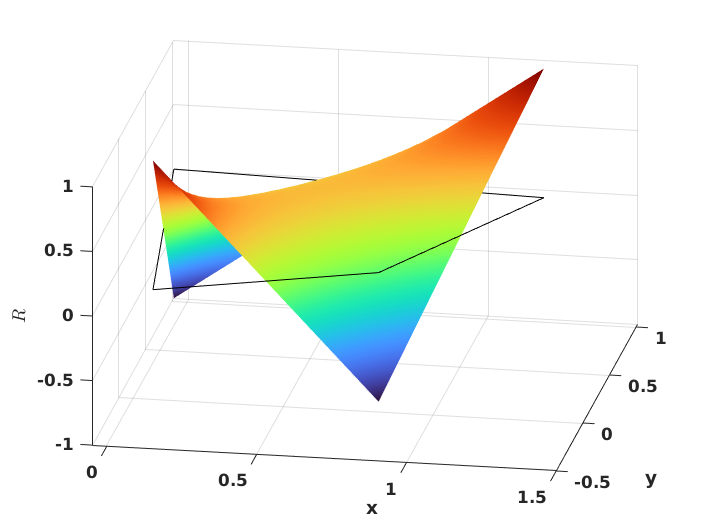
\includegraphics[width=5.5cm,height=4cm]{chapters/pics/R_1.png}
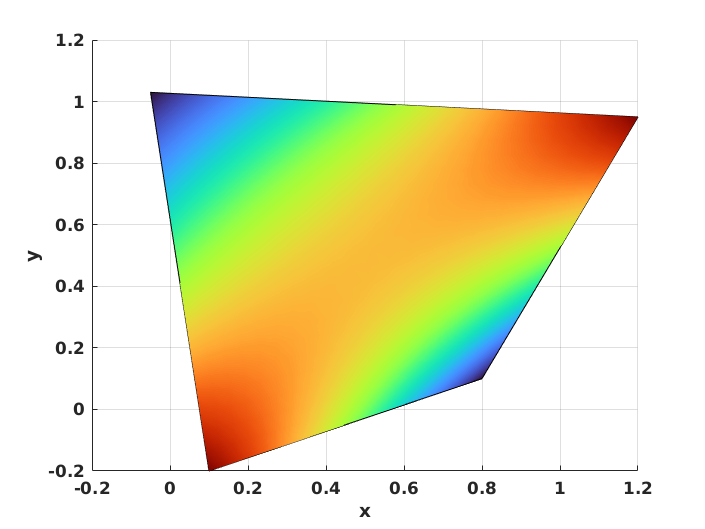
\includegraphics[width=5.5cm,height=4cm]{chapters/pics/R_2.png}
		  \caption{Rational function in $\mathcal{DS}_1$.}
		  \label{fig:rationalds1}
\end{figure}

We define vertex nodal basis function accordingly as
\begin{equation}\label{eq:vertexbasisds1}
\psi_{v,i}(\mathbf{x}) = \frac{\lambda_{d,m}(\mathbf{x}) - \frac{1}{2}\lambda_{d,m}(\mathbf{x}_{v,i+2})(1+ (-1)^i R(\mathbf{x}))}
{\lambda_{d,m}(\mathbf{x}_{v,i}) - \lambda_{d,m}(\mathbf{x}_{v,i+2})},
\end{equation}
where $m\equiv i+1 \Mod{2}$, and index $i$ is understood in the sence of modulo of $4$.
In Figure~\ref{fig:vertexbasisds1}, we show the vertex nodal basis function $\varphi_{v,0}$ in $\mathcal{DS}_1$ on a 
general quadrilateral, which evaluates $1$ at vertex $v_0$ and $0$ at other vertex.
\begin{figure}[ht]
\centering\small
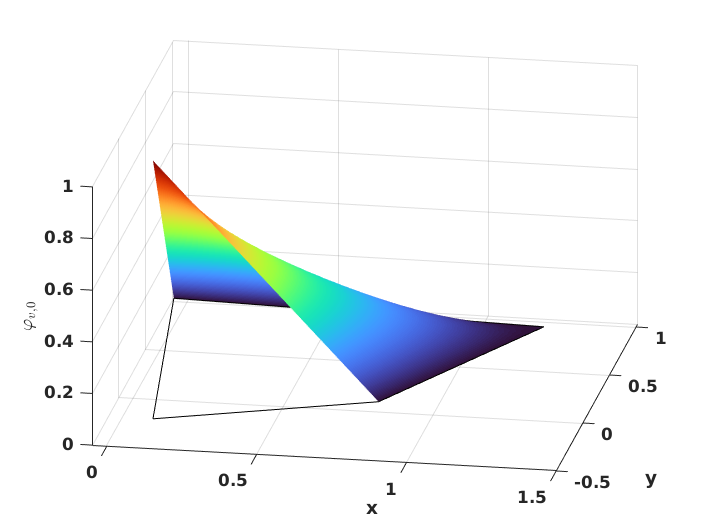
\includegraphics[width=5.5cm,height=4cm]{chapters/pics/phivds1_1.png}
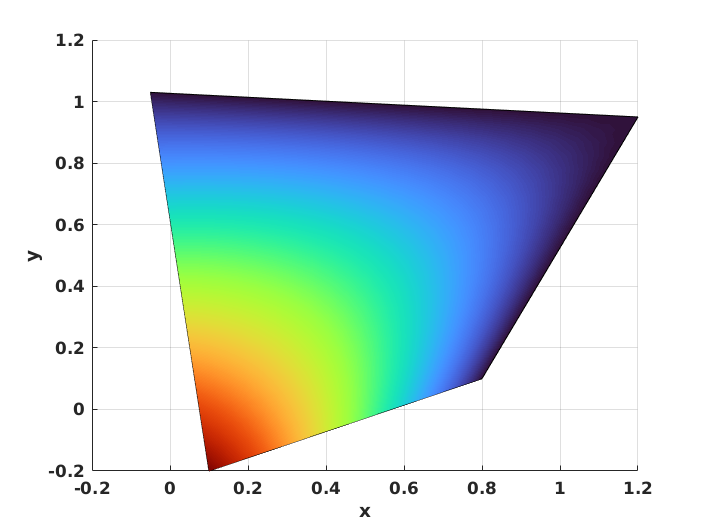
\includegraphics[width=5.5cm,height=4cm]{chapters/pics/phivds1_2.png}
		  \caption{Vertex nodal basis function  in $\mathcal{DS}_1$.}
		  \label{fig:vertexbasisds1}
\end{figure}

\begin{lem}\label{lem:interpolationop}
		  There exists a bounded interpolation operator $\mathcal{p}_h:W_p^l(E) \rightarrow \mathcal{DS}_r$ by
		  \begin{equation}\label{eq:interpolationop}
					 \mathcal{I}_h^rv(\mathbf{x}) \sum_{i=1}^{N_r} 
		  \end{equation}
\end{lem}

\begin{lem}\label{lem:approximation}
		  Under the asumptions of~\ref{lem:interpolationop}, there exists a 
		  constant $C = C(r, \sigma_*) > 0$ such that for all functions 
		  $v \in W_{l,p}(E^*)$, with $1\leq p \leq \infty$ and $l>1/p$ or 
		  ($l\geq 1$ if $p=1$),
		  \begin{equation}\label{eq:brambleHilbertDS}
					 \norm{v-\mathcal{I}_h^r}_{W_{m,p}} \leq C h_E^{l-m}
					 \lvert v \rvert_{W_{l,p}(E^*)}, \quad 0 \leq m \leq \text{min}(l,r+1).
		  \end{equation}
\end{lem}
